% Unofficial University of Cambridge Poster Template
% https://github.com/andiac/gemini-cam
% a fork of https://github.com/anishathalye/gemini
% also refer to https://github.com/k4rtik/uchicago-poster



\documentclass[final]{beamer}

% ====================
% Packages
% ====================

\usepackage[T1]{fontenc}
\usepackage{lmodern}
\usepackage[orientation=portrait,size=a0,scale=1.0]{beamerposter}
\usetheme{gemini}
\usecolortheme{nott}
\usepackage{graphicx}
\usepackage{booktabs}
\usepackage{tikz}
\usepackage{pgfplots}
\pgfplotsset{compat=1.14}
\usepackage{anyfontsize}
% ====================
% Lengths
% ====================

% If you have N columns, choose \sepwidth and \colwidth such that
% (N+1)*\sepwidth + N*\colwidth = \paperwidth
\newlength{\sepwidth}
\newlength{\colwidth}
\setlength{\sepwidth}{0.025\paperwidth}
\setlength{\colwidth}{0.45\paperwidth}

\newcommand{\separatorcolumn}{\begin{column}{\sepwidth}\end{column}}

% ====================
% Title
% ====================

\title{Segment and test approach on transport for hamiltonian systems}

\author{André Farinha \inst{1,2} \and Iberê Caldas \inst{1} \and Yves Elskens \inst{2}}

\institute[shortinst]{\inst{1} Universidade de São Paulo, São Paulo, Brazil \\ \inst{2} Aix-Marseille Université, Marseille, France}

% ====================
% Footer (optional)
% ====================

\footercontent{
  \href{https://github.com/Farinha96br/git_douts}{github repository: https://github.com/Farinha96br/git\_douts} \hfill
  JJD  2023, Marseille \hfill
  \href{farinha96br@gmail.com}{farinha96br@gmail.com}}
% (can be left out to remove footer)


% ====================
% Logo (optional)
% ====================

% use this to include logos on the left and/or right side of the header:
\logoright{
\includegraphics[height=7cm]{logos/logo_amu_rvb fond transparent.png}}
\logoleft{
\includegraphics[height=8cm]{logos/ifusp2.png}}

% ====================
% Body
% ====================

\begin{document}

% Refer to https://github.com/k4rtik/uchicago-poster
% logo: https://www.cam.ac.uk/brand-resources/about-the-logo/logo-downloads
% \addtobeamertemplate{headline}{}
% {
%     \begin{tikzpicture}[remember picture,overlay]
%       \node [anchor=north west, inner sep=3cm] at ([xshift=-2.5cm,yshift=1.75cm]current page.north west)
%       {\includegraphics[height=7cm]{logos/unott-logo.eps}}; 
%     \end{tikzpicture}
% }

\begin{frame}[t]
\begin{columns}[t]
\separatorcolumn
\begin{column}{\colwidth}

\begin{block}{Anomalous transport and how to identify it}
    

  Given a number $N$ of initial conditions in a system, we can categorize the transport, or diffusion, regime according to the mean square displacement

  \begin{equation}
    \sigma^2 (t) = \frac{1}{N} \sum_{N}^{i = 1}|\vec{x}_i(t) - \vec{x}_i(t_0)|^2 \approx 2Dt^\gamma.
    \label{msd}
  \end{equation}

  \begin{table}
    \begin{tabular}{c|c|c}
        subdiffusive & diffusive & superdiffusive\\
        $\gamma < 1$ & $\gamma = 1$ & $\gamma > 1$
    \end{tabular}
\end{table} 

The nature of what causes the anomalous transport is a complex discussion, but, when speaking of discrete maps, say $f$, the presence of periodic regions that have a behavior like $f_{n+1} \approx f_{n} + L \rightarrow f_N \approx f_{0} + NL$ causes anomalous transport, because when a trajectory sticks close to this orbit, it performs long flights.

\end{block}

\begin{block}{The standard map}
  The standard map is a discrete time system that represents a kicked rotator
  \begin{equation}
    p_{n+1} = p_n + K\sin(\theta_n) \hspace{1cm},\hspace{1cm} \theta_{n+1} = \theta_n + p_{n+1} \hspace{1cm} \textnormal{mod}(2\pi)
  \end{equation}

  As the parameter $K$ increases, we get different phase spaces, as shown in figure \ref{pspace}, where we notice the transition from a fully periodic phase space, to a mixed one, with $p$ bounded; then, as $K$ increases further, $p$ becomes unbounded, for $K > K_c \approx 0.9716$ where the last invariant line is broken.

  \begin{figure}
    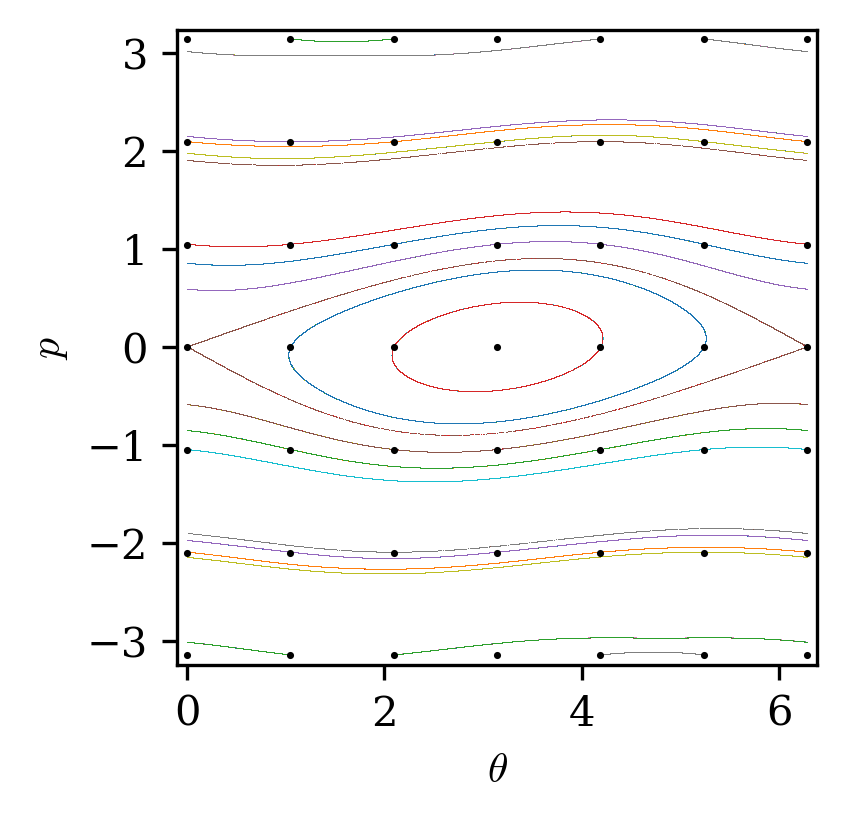
\includegraphics[width = 0.3\textwidth]{map_1_0.2000.png}
    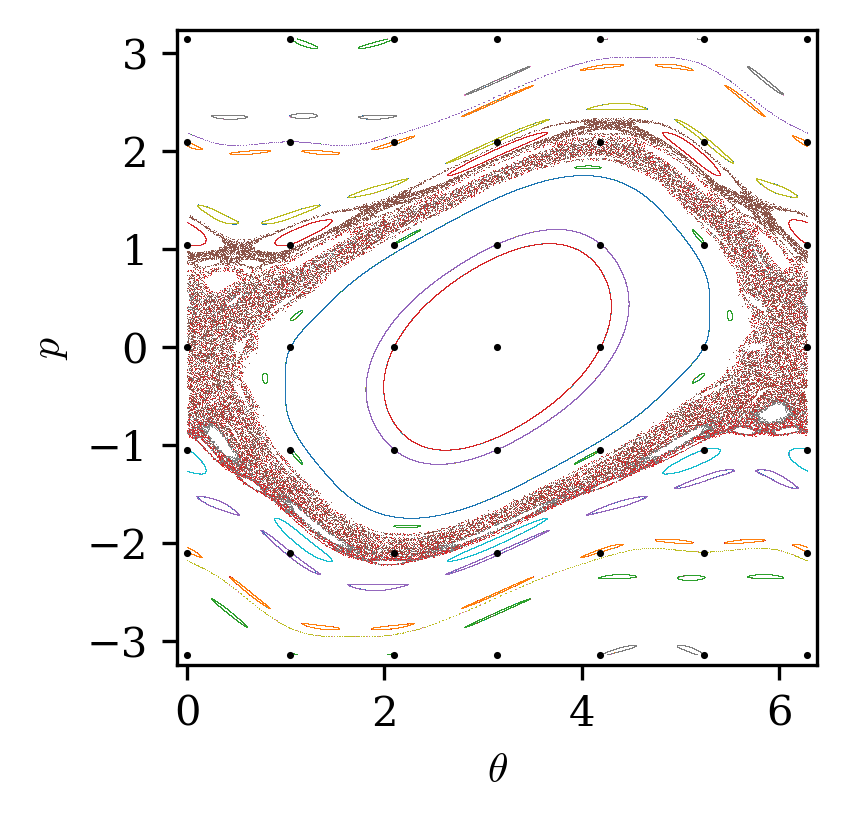
\includegraphics[width = 0.3\textwidth]{map_1_0.9000.png}
    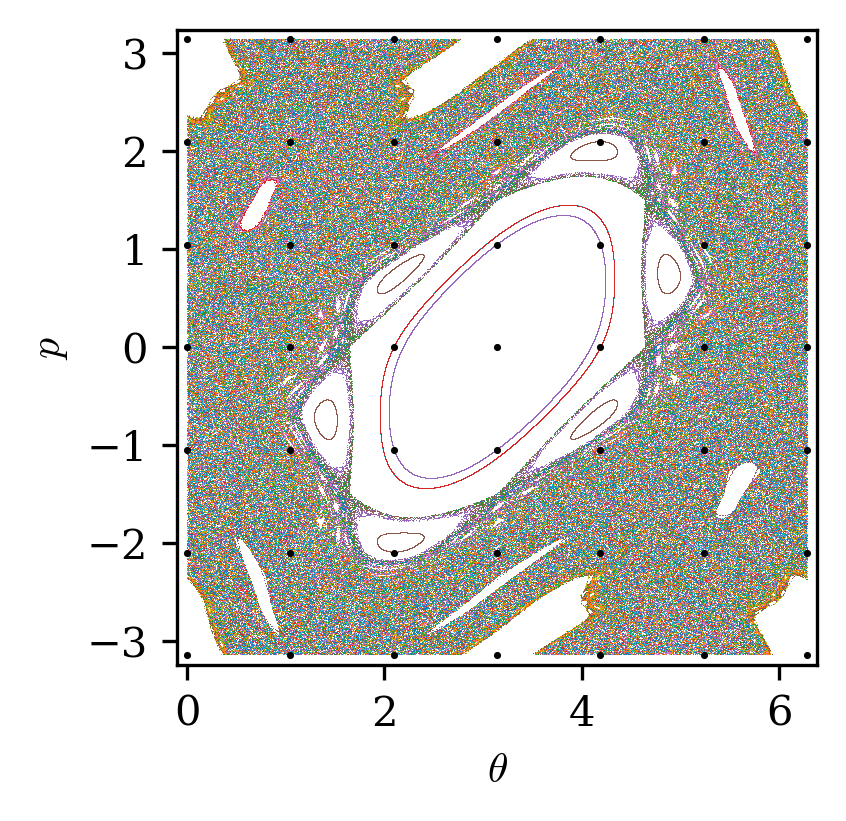
\includegraphics[width = 0.3\textwidth]{map_1_1.5000.png}
    \caption{Phase space for $K=0.2$ (left), $0.9$ (middle) and $1.5$ (right).}
    \label{pspace}
  \end{figure}

  Thus for $K < K_c$ we have $\gamma = 0$, because no large scale transport is present in $p$. For $K > K_c$ we start to see some transport, but normal diffusion only appears for $K \gtrsim 1.2$, and then superdiffusion for some values of $K$ as we see on figure \ref{areas}, due do the existence of accelerator modes; that is, for some initial conditions $(\theta_0,p_0)$ we get
  
  \begin{equation}
    p_{n} \approx p_0 + an \hspace{1cm},\hspace{1cm} \theta_{n} \approx \frac{an^2}{2} \hspace{1cm} 
  \end{equation}

  It is worth noticing that, for the evaluation of $\gamma$ on figure \ref{areas}, we used $10^4$ initial conditions, each iterated \textit{costing}  over $5\times10^4$. This leads to $5\times 10^8$ step operations per data point.

\end{block}
  
\begin{block}{Novel segment and test approach}
 The approach consists in creating a somewhat dense Poincaré section, of a system with mixed phase space. We segment the chaotic and periodic regions, and use a single initial condition to identify the regime on each region and check the existence of accelerator modes. The standard map was chosen as a benchmark for the method since it is much studied in the literature.

  The regimes present in the standard map are \textbf{Periodic confined (PC)}, \textbf{Bounded chaotic (BC)}, \textbf{Unbounded chaotic (UC)} and \textbf{Periodic accelerated (PA)}.

  The choice of using a morphological approach was made due to its flexibility and robustness. The method is also tunable for different problems. The initial data for the map were created using $81$ initial conditions spread evenly on the phase space, and each iterated for the same $5\times 10^4$, as used to evaluate $\gamma$, so each data point \textit{costed} around $10^5$ step operations, being much cheaper than the usual approach.

  Here we sampled the map as a $1024\times1024$ grid, the structuring element for dilations and erosion was a disk with a radius of 2 pixels. 

  \begin{figure}
    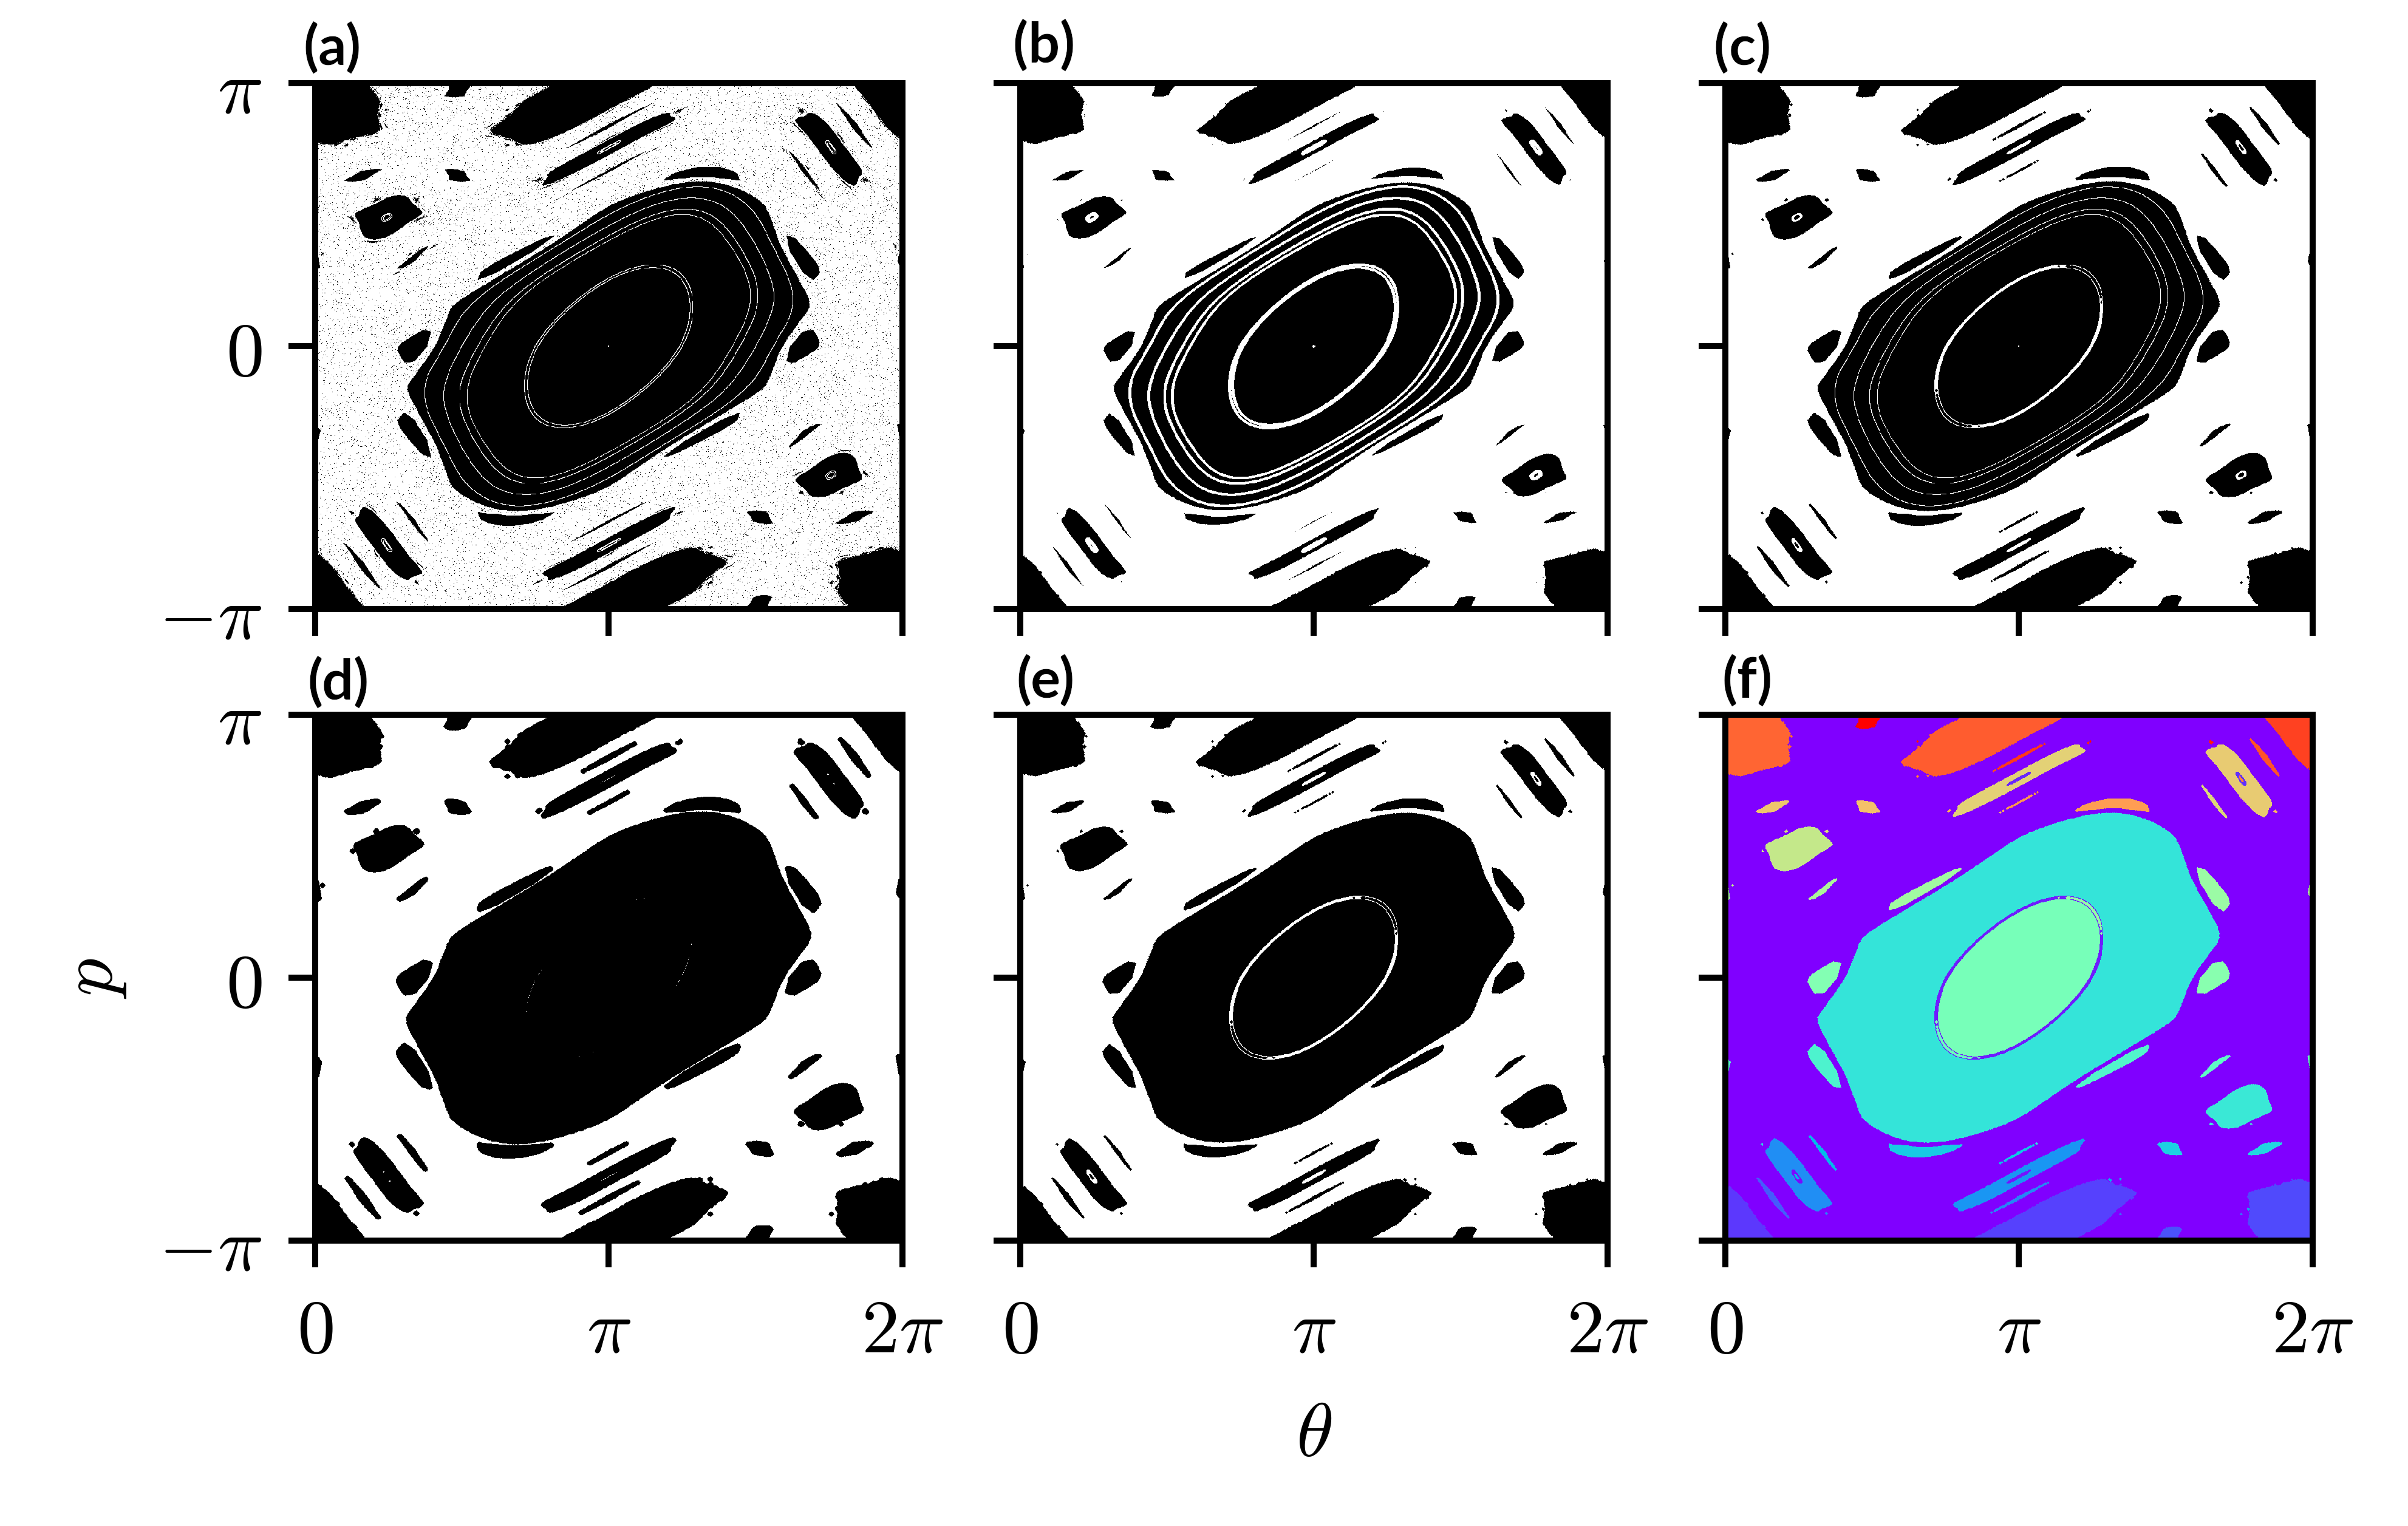
\includegraphics[width = 1.0\textwidth]{mm_6_2.png}
    \caption{The morphological steps to segment the regions of interest: sampling of the map (a); dilation (b); erosion (c); erosion (d); reconstruction (e); segmented regions (f) for $K = 1.2$}
  \end{figure}

\end{block}



\end{column}
 
\separatorcolumn
\begin{column}{\colwidth}

   \begin{block}{Results on standard map}

    Figure \ref{label} shows the 4 regimes of transport correctly classified: green (PC), yellow (BC), blue (UC) and magenta (PA).

    \begin{figure}
      \centering
      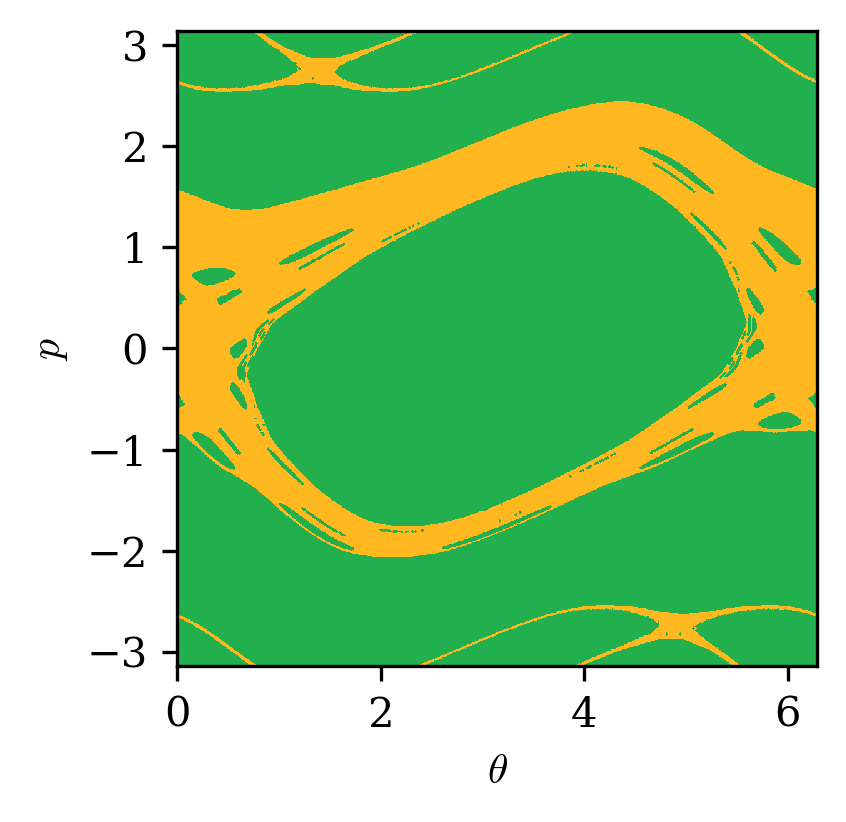
\includegraphics[width = 0.3\textwidth]{label_000.8127.png}
      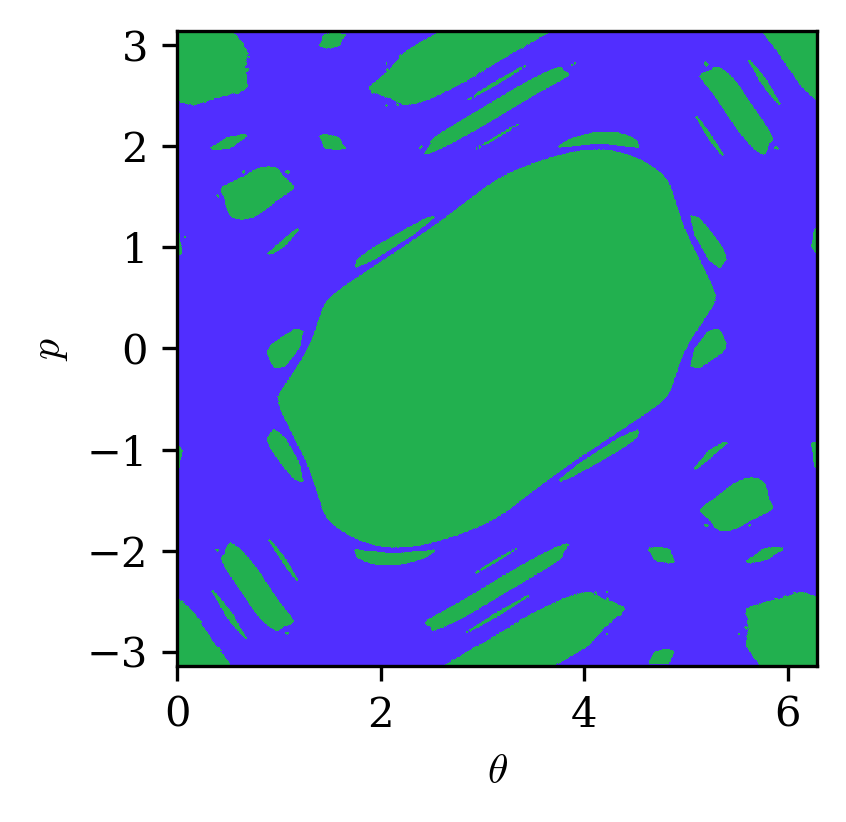
\includegraphics[width = 0.3\textwidth]{label_001.2040.png}
      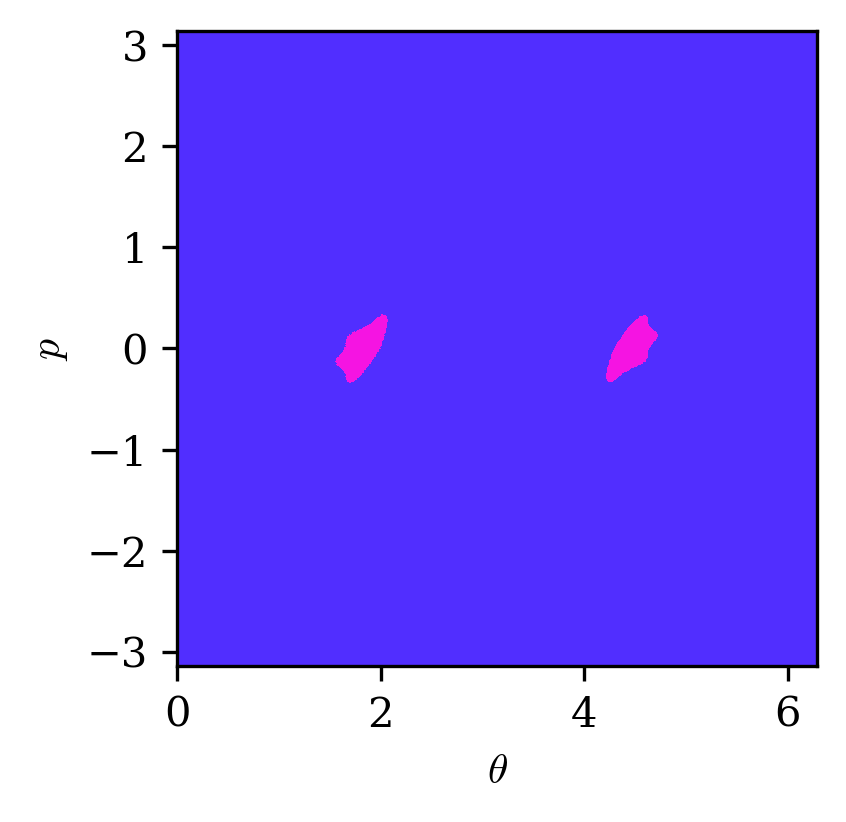
\includegraphics[width = 0.3\textwidth]{label_006.5318.png}
      \caption{The four types of regimes classified for $K=0.8127$ (left), $1.2040$ (middle) and $6.5318$ (right).}
      \label{label}
  \end{figure}

 We notice how the transport regime changes close to $K_c$, as well as the presence of superdiffusive regime where accelerator modes are present.


  \begin{figure}
    \centering
    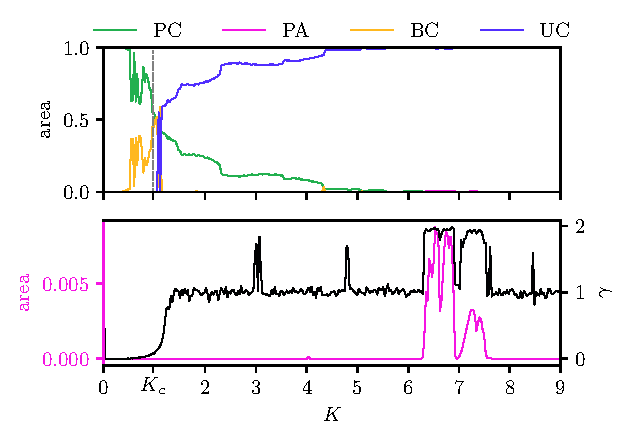
\includegraphics[width = 0.7\textwidth]{areas.pdf}
    \caption{Top: Fractional area of each regime; Bottom: Comparison between the accelerator modes area (magenta), and the exponent $\gamma$ (black)}
    \label{areas}
\end{figure}

  
  \end{block}

  \begin{block}{In progress}
    As the method has been tested in a well known system, it is now being applied to a nonintegrable model of electric drift in a 2-wave plasma system
    
    \begin{equation}
      H(x,y,t) = \phi_o - v_1x + A_1 \sin(k_{x1}x)\cos(k_{y1}y) + \underset{\uparrow}{A_2}\sin(k_{x2}x + \underset{\uparrow}{\theta_x}\cos(k_{y2}(y - vt)).
    \end{equation}

    When $\phi_o - v_1x = 0$, for some values of $A_2$ and $\theta_x$, ballistic modes are present, which cause anomalous transport, and we see on figure \ref{paramspace} for which parameters superdiffusion is present.
 
    \begin{figure}
      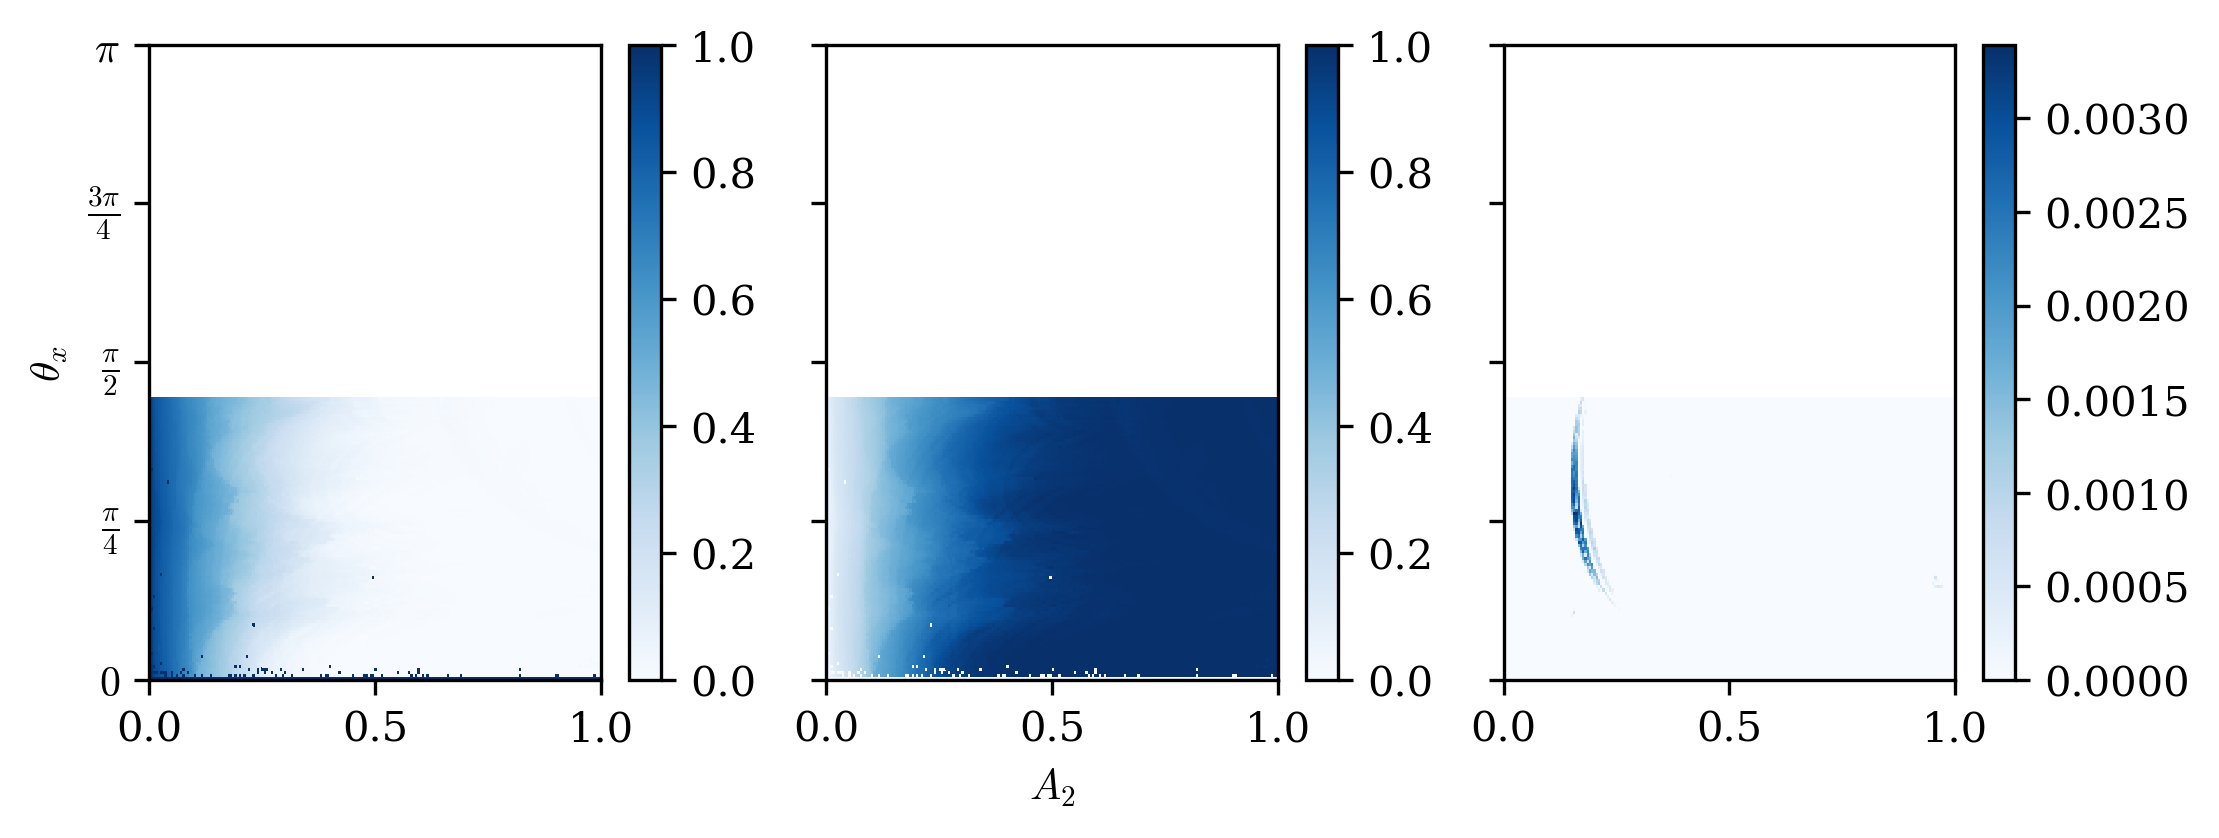
\includegraphics[width = 0.9\textwidth]{paramspace.png}
      \caption{Fractional areas for trapped (left), diffusive (middle) and ballistic (right) regimes.}
      \label{paramspace}
    \end{figure}
    
  \end{block}


  \begin{block}{Conclusions}
    With these results we were able to identify the presence of anomalous transport of momentum in the standard map using the segment and test approach. The values of $K$ where the method could not identify the anomalous transport, may be related to the accelerator modes being smaller than the structuring elements of the operations, or than the pixels themselves. This method is also interesting, as a cheap exploratory tool to identify superdiffusion since the existence of accelerator modes and like are a sufficient but not necessary condition. 
    
  \end{block}



  \begin{block}{Main references}

    \nocite{chirikov1979universal,gonzales1987digital,ishizaki1991anomalous,klages2008anomalous}
    \footnotesize{\bibliographystyle{ieeetr}\bibliography{poster}}



  \end{block}

  


\begin{block}{Acknowledgements}
  \begin{figure}
      \centering
      
\includegraphics[height = 4cm]{logos/capes logo.png}
      
\includegraphics[height = 4cm]{logos/Logo-CNRS.png}
      
\includegraphics[height = 4cm]{logos/mesocentre.png}
      
\includegraphics[height = 4cm]{logos/PIIM_redondo(1).png}
      
\includegraphics[height = 4cm]{logos/cnpq.png}
      
\includegraphics[height = 4cm]{logos/fapesp.png}
      
\includegraphics[height = 4cm]{logos/ufpr.png}
      
\includegraphics[height = 4cm]{cofecubp.jpg}
  \end{figure}
    
\end{block}

 

\end{column}
 


\end{columns}
\end{frame}

\end{document}